\section{Real-time analysis}
\label{rta}
HEP and industry share a common challenge—the rapid processing of large quantities of data. \cite{hu-big-data} Recent advances in computing, in particular in the areas of machine learning and hybrid architectures, have enabled the possibility of processing data in real-time, i.e. as data is collected (also commonly referred to as ``online'' processing). \cite{real-time-computing} By processing data online, resources (computing power, storage space, energy, etc.) can be saved and further insights can be obtained from the data recorded, as shown in Figure~\ref{rta-diagram}. \par

\begin{figure*}[h!]
    \centering
    % Use the relevant command for your figure-insertion program
    % to insert the figure file. See example above.
    % If not, use
    %\vspace*{5cm}       % Give the correct figure height in cm
    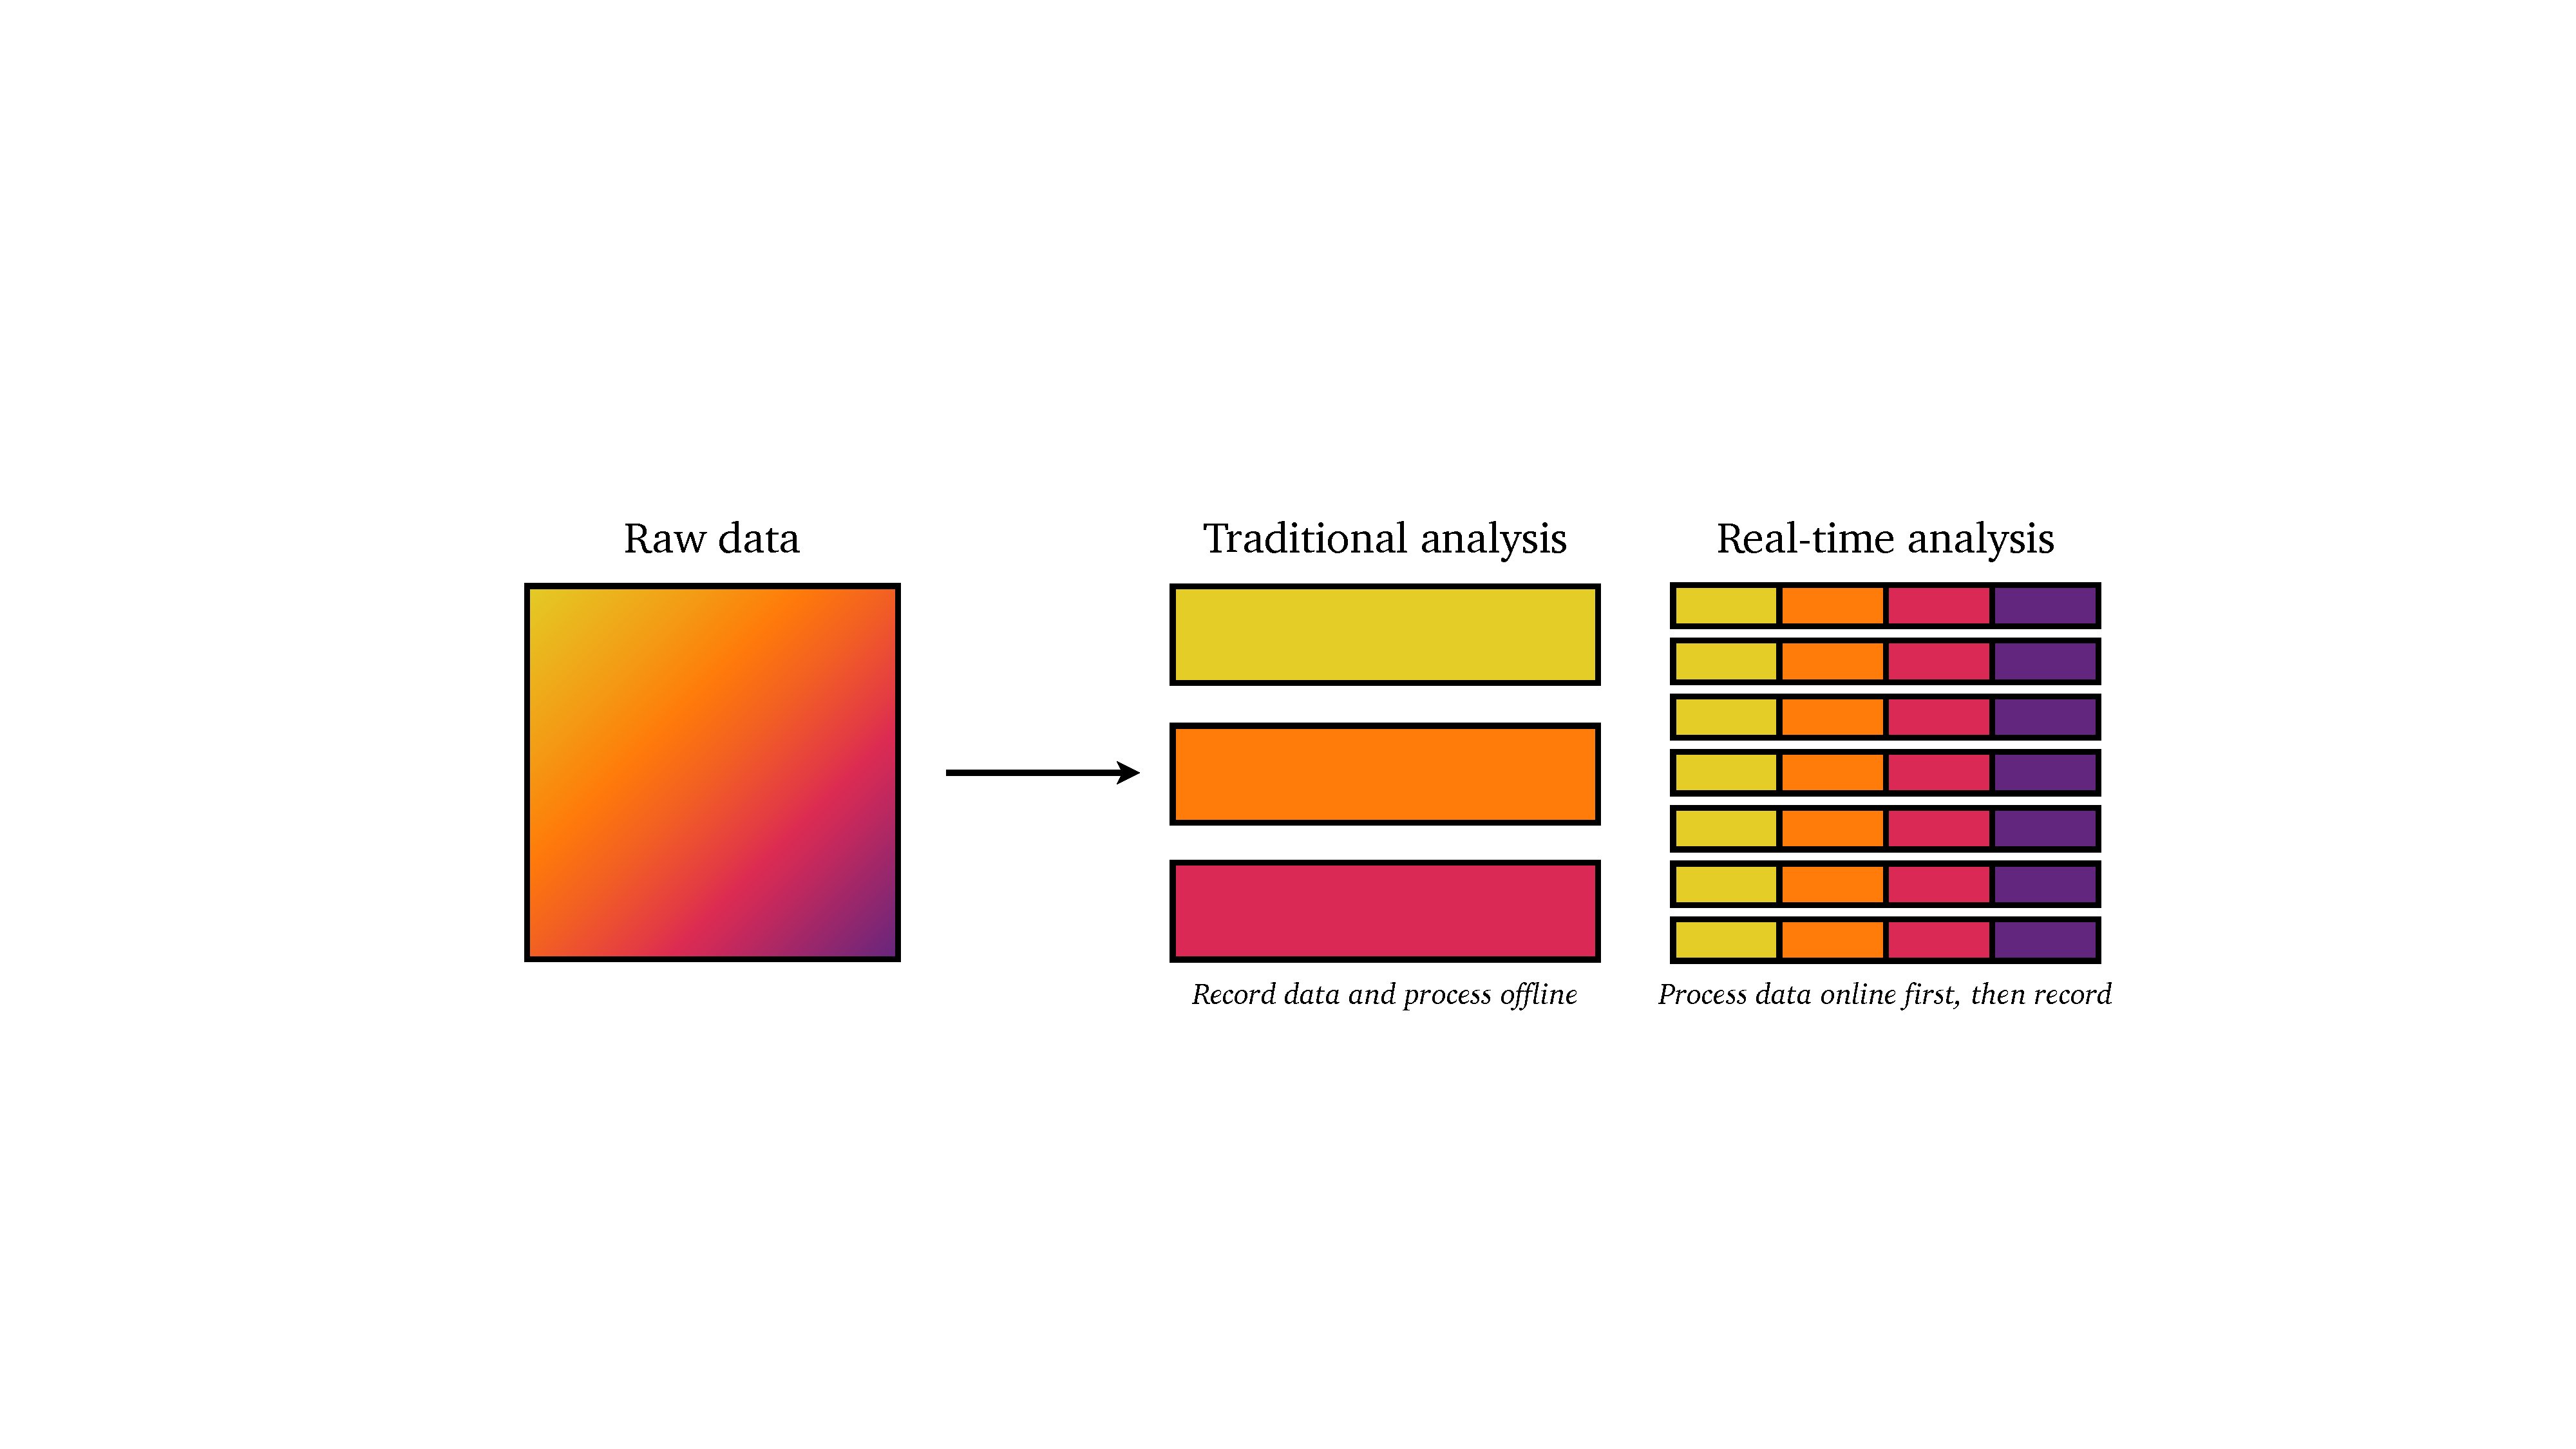
\includegraphics[width=\linewidth]{/Users/jgooding/Documents/SMARTHEP/CHEP2023/CHEP2023/proceedings/figures/rta-diagram.pdf}
    \caption{Traditional and RTA approaches to data processing. Traditional approaches rely on recording all data and processing this offilne; in RTA, data is processed as it is produced, recording only the relevant portions, enabling greater volumes of processed data to be stored.}
    \label{rta-diagram}       % Give a unique label
\end{figure*}

RTA techniques have seen widespread adoption across HEP, in particular amongst trigger and data acquisition (TDAQ) systems. Since it is not possible to record a full detector readout and carry out event reconstruction at the LHC collision rate of {40}{ MHz}, triggers must be devised to select only those events relevant to the physics goals of an experiment. Such triggers conventionally consist of a hardware system making coarse decisions from partial detector readout, and a staged software trigger, applying gradually more finely-grained selections with increasingly more detailed reconstructions of events.\par

%In industry, the limitations of the scale of ``big data'' looms over many applications of computing. However, \par


\subsection{Machine learning}
\label{machine-learning}
ML, a catch-all term for a family of techniques and technologies wherein algorithms are trained to analyse data, enables rapid decision-making and pattern recognition across a broad range of use cases. \cite{intro-ml} In HEP, the adoption of ML began with classifiers for offline physics analysis, since widening to a variety of classification and pattern recognition/anomaly detection techniques for use online and offline. \cite{albertsson-ml}\par

ML classifiers are algorithms classed with classification, with Boosted Decision Trees (BDTs) and Neural Networks (NNs) amongst those most commonly employed in HEP. The use of BDTs in signal selection for offline physics analysis has become standard practice, e.g. suppresion of combinatorial background in the LHCb experiment measurement of the $B_s^0-\bar{B}_s^0$ oscillation frequency. \cite{delta-ms} Classifiers can also aid tasks such as event reconstruction, e.g. the CMS boosted event shape tagger, a NN trained to discriminate between possible $t$, $W^\pm$, $Z^0$ and $H$ candidates within an event. \cite{CMS-best} In industry, ML classifiers are used frequently in content deliver\par

ML techniques can also be applied to pattern recognition and anomaly detection—tasks which cannot be realistically carried out on the scales of data presently being analysed. In industry, this is applied intuitively to fraud detection, wherein even subtle changes in transaction  data can indicate fraudulent activity. In HEP, such anomaly detection can be applied to searches, for example the ATLAS search for resonant decays to a Higgs boson. \cite{anomaly-hep}

\subsection{Hybrid architectures}
\label{hybrid-architectures}
Typical computational resources consist of Central Processing Units (CPUs), processors which are designed for general purpose computation (i.e. varied tasks with significant variety in computing/memory resources), with large on-board memory and often multiple processing cores. Alternative computing architectures, such as Graphical Processing Units (GPUs) and Field-programmable gate arrays (FPGAs) shown in Figure~\ref{architectures}, can be applied in conjunction or in place of CPU architectures to accelerate processing where tasks are not well-suited to CPU architectures alone. \par

\begin{figure*}[h!]
    \centering
    % Use the relevant command for your figure-insertion program
    % to insert the figure file. See example above.
    % If not, use
    %\vspace*{5cm}       % Give the correct figure height in cm
    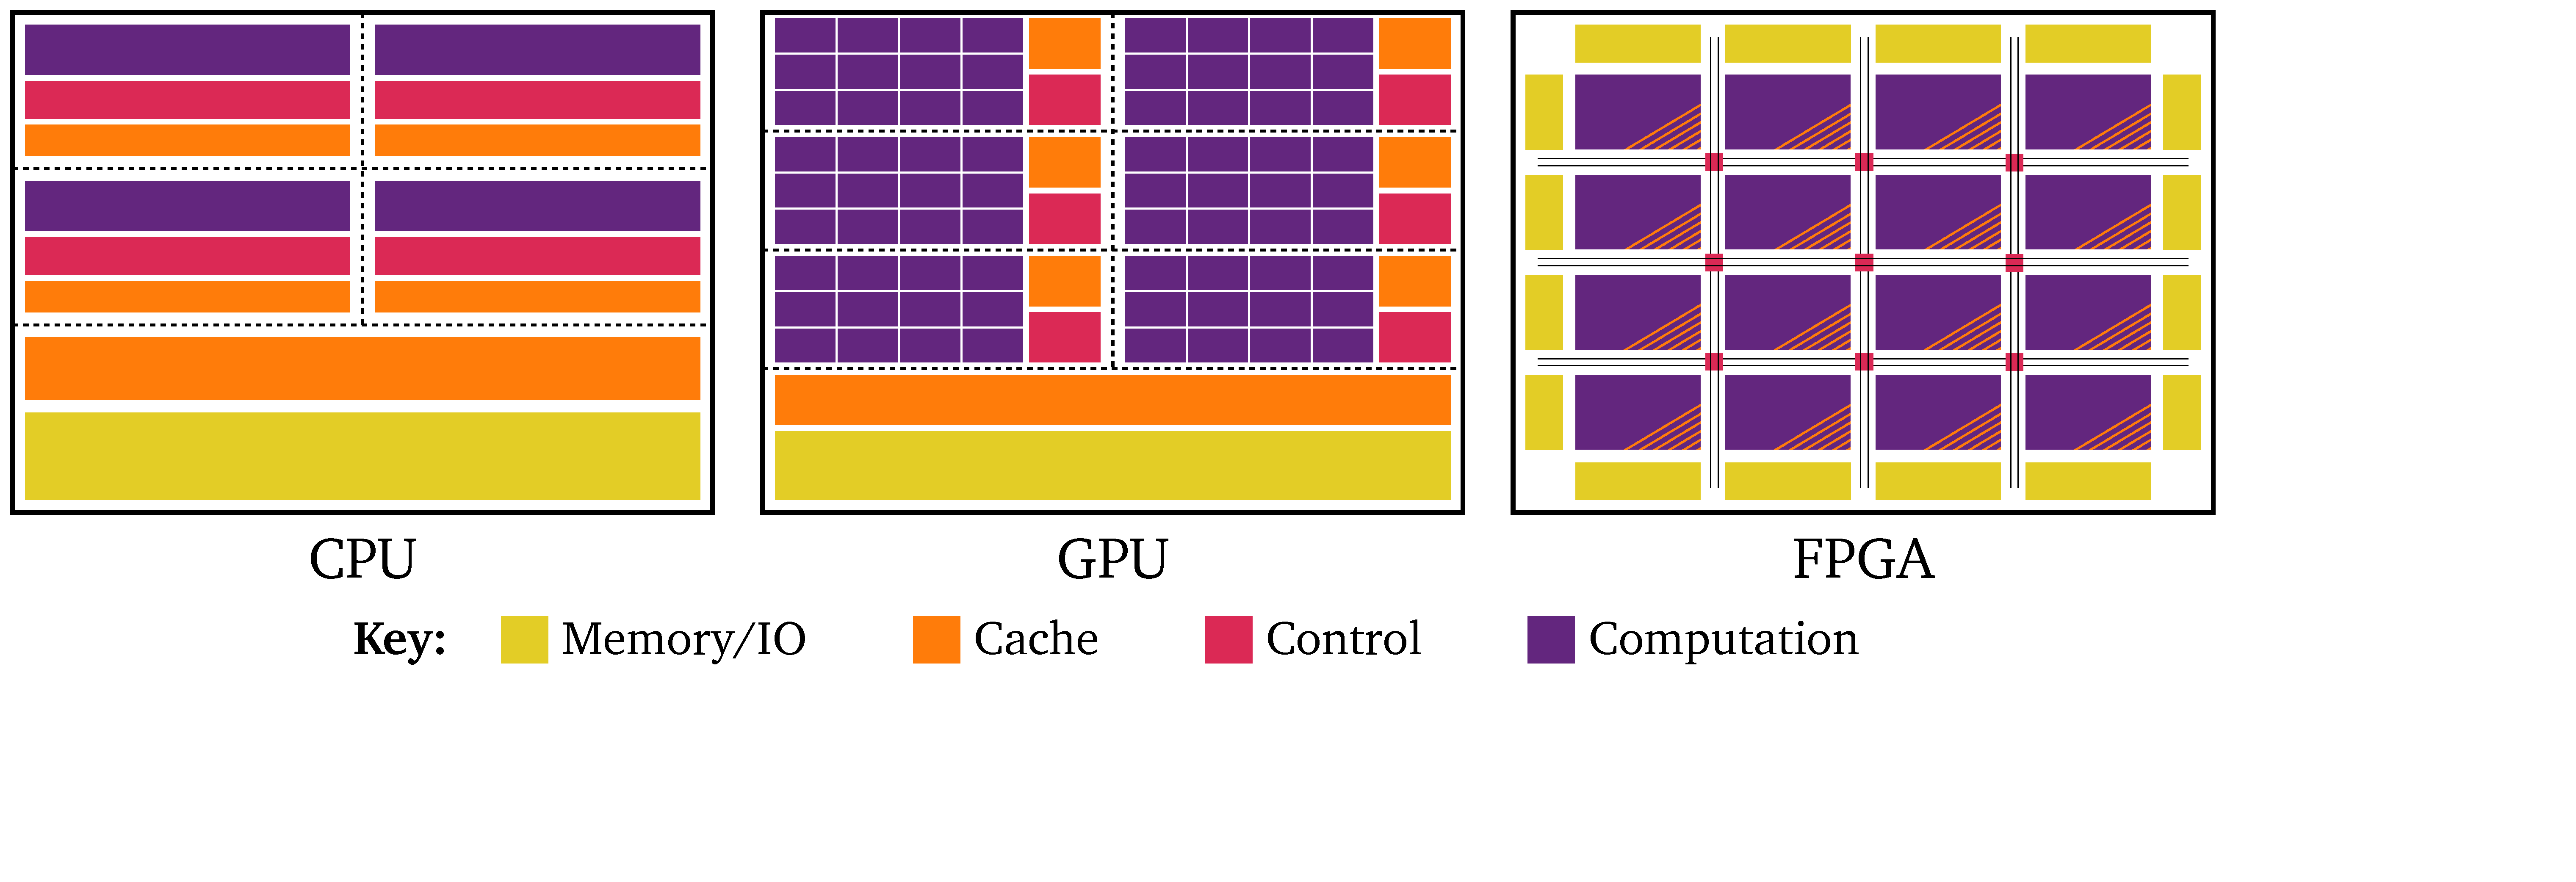
\includegraphics[width=\linewidth,clip]{/Users/jgooding/Documents/SMARTHEP/CHEP2023/CHEP2023/proceedings/figures/architectures-diagram.pdf}
    \caption{Comparison of CPU, GPU and FPGA architectures. A CPU is typically formed of several cores (each containing computational, control and cache resources) and centralized cache, memory and input/output (IO) interface. GPUs contain similar centralized resources, though consist of many multiprocessors, each containing a greater proportion of computational resources than a CPU core. GPU multiprocessors are also themselves partitioned to perform tasks in parallel. FPGAs are structured rather differently with memory and IO connected to many interlinked control blocks formed of simpler logic gate arrangements, often accompanied by a small cache.}
    \label{architectures}       % Give a unique label
\end{figure*}

GPUs typically contain many more computing units than CPUs, providing better performance in highly parallelisable tasks. This makes GPUs well-suited to accelerating event processing, which consists of many similar but computationally intensive tasks such as cluster finding and track fitting. \cite{vomBruch-gpus} For less computationally intensive tasks, FPGAs (integrated circuits which can be programmed for specific tasks) can be employed. \cite{fpgas-intro} Examples of such tasks include low-level trigger decisions, which typically consist of simple selections but must be made rapidly. \cite{duarte-fpgas}\par